\begin{figure}[htbp]
\centering
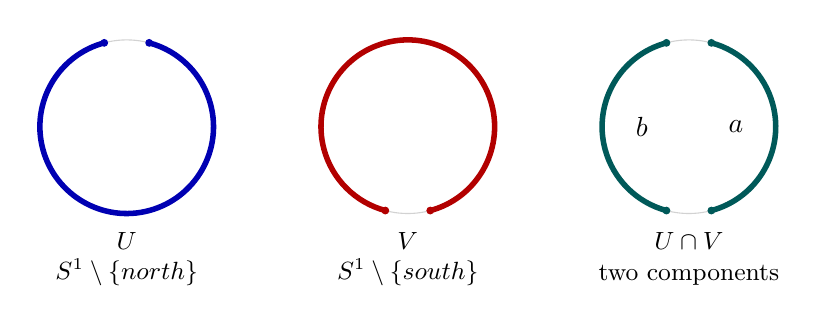
\begin{tikzpicture}[scale=1.05]
\begin{scope}[xshift=-3.4cm]
\draw[gray!35] (0,0) circle (1.05);
\draw[blue!70!black,line width=2pt] (105:1.05) arc (105:435:1.05);
\draw[fill=white,blue!70!black] (105:1.05) circle (.04) (75:1.05) circle (.04);
\node[align=center,font=\small] at (0,-1.6) {$U$\\$S^1\setminus\{\text{north}\}$};
\end{scope}
\begin{scope}
\draw[gray!35] (0,0) circle (1.05);
\draw[red!70!black,line width=2pt] (-75:1.05) arc (-75:255:1.05);
\draw[fill=white,red!70!black] (-75:1.05) circle (.04) (255:1.05) circle (.04);
\node[align=center,font=\small] at (0,-1.6) {$V$\\$S^1\setminus\{\text{south}\}$};
\end{scope}
\begin{scope}[xshift=3.4cm]
\draw[gray!35] (0,0) circle (1.05);
\draw[teal!70!black,line width=2pt] (-75:1.05) arc (-75:75:1.05);
\draw[teal!70!black,line width=2pt] (105:1.05) arc (105:255:1.05);
\foreach \a in {-75,75,105,255} \draw[fill=white,teal!70!black] (\a:1.05) circle (.04);
\node at (-.57,0) {$b$};\node at (.57,0) {$a$};
\node[align=center,font=\small] at (0,-1.6) {$U\cap V$\\two components};
\end{scope}
\end{tikzpicture}
\caption{Two punctured-circle open arcs cover $S^1$. Gaps are enlarged
schematically to show the omitted poles. Their overlap has a left and a
right component; a locally constant function chooses two independent values.}
\label{fig:mayer-vietoris-circle}
\end{figure}
